% !TEX TS-program = XeLaTeX
% use the following command:
% all document files must be coded in UTF-8
\documentclass[portuguese]{textolivre}
% build HTML with: make4ht -e build.lua -c textolivre.cfg -x -u article "fn-in,svg,pic-align"

\journalname{Texto Livre}
\thevolume{15}
%\thenumber{1} % old template
\theyear{2022}
\receiveddate{\DTMdisplaydate{2022}{1}{25}{-1}} % YYYY MM DD
\accepteddate{\DTMdisplaydate{2022}{2}{3}{-1}}
\publisheddate{\DTMdisplaydate{2022}{2}{25}{-1}}
\corrauthor{Ronaldo Corrêa Gomes Junior}
\articledoi{10.35699/1983-3652.2022.38008}
%\articleid{NNNN} % if the article ID is not the last 5 numbers of its DOI, provide it using \articleid{} commmand
\runningauthor{Gomes Junior et al.} 
%\editorname{Leonardo Araújo} % old template
\sectioneditorname{Daniervelin Pereira}
\layouteditorname{Leonado Araújo}

\title{Tecnologias digitais para aprender e ensinar inglês no Brasil}
\othertitle{Digital technologies to learn and teach English in Brazil}
% if there is a third language title, add here:
%\othertitle{Artikelvorlage zur Einreichung beim Texto Livre Journal}

\author[1]{Ronaldo Corrêa Gomes Junior \orcid{0000-0003-4165-8629} \thanks{Email: \url{ronaldocgomes@gmail.com}}}
\author[1]{Luciana de Oliveira Silva \orcid{0000-0001-8109-2389} \thanks{Email: \url{luciana.fale@gmail.com}}}
\author[1]{Vera Lúcia Menezes de Oliveira e Paiva \orcid{0000-0001-9379-5698} \thanks{Email: \url{vlmop@veramenezes.com}}}
\affil[1]{Universidade Federal de Minas Gerais, Faculdade de Letras, Belo Horizonte, MG, Brasil.}

\addbibresource{article.bib}
% use biber instead of bibtex
% $ biber article

% used to create dummy text for the template file
\definecolor{dark-gray}{gray}{0.35} % color used to display dummy texts
\usepackage{lipsum}
\SetLipsumParListSurrounders{\colorlet{oldcolor}{.}\color{dark-gray}}{\color{oldcolor}}

% used here only to provide the XeLaTeX and BibTeX logos
\usepackage{hologo}

% if you use multirows in a table, include the multirow package
\usepackage{multirow}

% provides sidewaysfigure environment
\usepackage{rotating}

% CUSTOM EPIGRAPH - BEGIN 
%%% https://tex.stackexchange.com/questions/193178/specific-epigraph-style
\usepackage{epigraph}
\renewcommand\textflush{flushright}
\makeatletter
\newlength\epitextskip
\pretocmd{\@epitext}{\em}{}{}
\apptocmd{\@epitext}{\em}{}{}
\patchcmd{\epigraph}{\@epitext{#1}\\}{\@epitext{#1}\\[\epitextskip]}{}{}
\makeatother
\setlength\epigraphrule{0pt}
\setlength\epitextskip{0.5ex}
\setlength\epigraphwidth{.7\textwidth}
% CUSTOM EPIGRAPH - END

% LANGUAGE - BEGIN
% ARABIC
% for languages that use special fonts, you must provide the typeface that will be used
% \setotherlanguage{arabic}
% \newfontfamily\arabicfont[Script=Arabic]{Amiri}
% \newfontfamily\arabicfontsf[Script=Arabic]{Amiri}
% \newfontfamily\arabicfonttt[Script=Arabic]{Amiri}
%
% in the article, to add arabic text use: \textlang{arabic}{ ... }
%
% RUSSIAN
% for russian text we also need to define fonts with support for Cyrillic script
% \usepackage{fontspec}
% \setotherlanguage{russian}
% \newfontfamily\cyrillicfont{Times New Roman}
% \newfontfamily\cyrillicfontsf{Times New Roman}[Script=Cyrillic]
% \newfontfamily\cyrillicfonttt{Times New Roman}[Script=Cyrillic]
%
% in the text use \begin{russian} ... \end{russian}
% LANGUAGE - END

% EMOJIS - BEGIN
% to use emoticons in your manuscript
% https://stackoverflow.com/questions/190145/how-to-insert-emoticons-in-latex/57076064
% using font Symbola, which has full support
% the font may be downloaded at:
% https://dn-works.com/ufas/
% add to preamble:
% \newfontfamily\Symbola{Symbola}
% in the text use:
% {\Symbola }
% EMOJIS - END

% LABEL REFERENCE TO DESCRIPTIVE LIST - BEGIN
% reference itens in a descriptive list using their labels instead of numbers
% insert the code below in the preambule:
%\makeatletter
%\let\orgdescriptionlabel\descriptionlabel
%\renewcommand*{\descriptionlabel}[1]{%
%  \let\orglabel\label
%  \let\label\@gobble
%  \phantomsection
%  \edef\@currentlabel{#1\unskip}%
%  \let\label\orglabel
%  \orgdescriptionlabel{#1}%
%}
%\makeatother
%
% in your document, use as illustraded here:
%\begin{description}
%  \item[first\label{itm1}] this is only an example;
%  % ...  add more items
%\end{description}
% LABEL REFERENCE TO DESCRIPTIVE LIST - END


% add line numbers for submission
%\usepackage{lineno}
%\linenumbers

\begin{document}
\maketitle

\begin{polyabstract}
\begin{abstract}
Em uma sociedade pós-industrial marcada pela ascensão das tecnologias da informação e comunicação e pela arquitetura em rede, investigações sobre os usos de recursos tecnológicos para ensinar e aprender línguas tornam-se cada vez mais importantes para conhecermos o estado de difusão dessas inovações. Este estudo em forma de \textit{survey on-line} buscou investigar quais eram as ferramentas digitais mais utilizadas por aprendizes e professores de inglês no Brasil. A investigação ocorreu em 2018 e 2019, antes da pandemia da Covid-19 (SARS-CoV-2), e contou com a participação de professores e estudantes de todas as regiões do Brasil. Os participantes responderam a um questionário divulgado em redes sociais e em eventos científicos da área de Letras. Os respondentes demonstraram identificar os diversos propiciamentos de recursos digitais para aprender e ensinar inglês.

\keywords{Ferramentas digitais \sep Ensino de inglês \sep Aprendizagem de inglês}
\end{abstract}

\begin{english}
\begin{abstract}
In a post-industrial society marked by the rise of information and communication technologies and networked architecture, investigations on the use of technological resources to teach and learn languages are becoming increasingly important to understand the state of diffusion of these innovations. This online survey aimed to investigate what digital tools are most used by English learners and teachers in Brazil. The investigation was carried out in 2018 and 2019, before the Covid-19 (SARS-CoV-2) pandemic, and the participants were teachers and students from all regions of Brazil. The participants completed a questionnaire announced in social networks and scientific events in the area of Arts. They demonstrated to identify affordances of digital resources to learn and teach English.

\keywords{Digital tools \sep English teaching \sep English learning}
\end{abstract}
\end{english}
% if there is another abstract, insert it here using the same scheme
\end{polyabstract}

\section{Introdução}\label{sec-intro}
Esta pesquisa precede um momento no tempo-espaço extremamente marcante na história da civilização. A pandemia da Covid-19 (SARS-CoV-2), anunciada oficialmente em 11 de março de 2020 pela Organização Mundial da Saúde \cite{who_who_2020}, acarretou mudanças drásticas em diversas esferas sociais, sendo a educacional uma das mais afetadas. De uma hora para outra, as atividades educacionais passaram a contar exclusivamente com as tecnologias digitais. Como destacam \textcite{braga_elephant_2021}, a pandemia vem acelerando o uso e a integração de tecnologias que até então vinham ocorrendo lentamente. Este esclarecimento é importante para marcar temporalmente o desenvolvimento desta pesquisa e para destacar que nossa análise se refere a um contexto pré-pandêmico, já que os dados foram coletados nos anos de 2018 e 2019.

O avanço das tecnologias influenciou a maneira como vivemos, nos comunicamos e aprendemos. Para \textcite{castells_sociedade_2006}, a revolução tecnológica propiciada pela ascensão das tecnologias da informação e comunicação influenciou o mundo de forma impactante, proporcionando a democratização do acesso à informação e o empoderamento dos indivíduos por meio de possibilidades reais de autoria. No entanto, sabemos que esse acesso não é tão democrático assim em sociedades com acentuadas desigualdades, pois os equipamentos são caros, nem sempre há Internet disponível e muito menos acesso gratuito. Em alguns lugares, não há sequer energia elétrica.

A sociedade pós-industrial, uma sociedade em rede, é marcada pela expansão e massificação do acesso à Internet, o que interfere significativamente em nossas vidas e muda as formas como interagimos no e com o mundo. Dessa maneira, é importante investigar as tecnologias utilizadas para ensinar e aprender línguas, de modo a lançar luz sobre esse aspecto importante em uma sociedade em rede.  
 
Este estudo foi realizado em um contexto pré-pandêmico, nos anos de 2018 e 2019, e fez parte de uma série de ações de pesquisa do Laboratório de Linguagem e Tecnologia (LALINTEC), composto por pesquisadores-professores da Universidade Federal de Minas Gerais (UFMG) e do Centro Federal de Educação Tecnológica de Minas Gerais (CEFET-MG). A pesquisa é um dos produtos de um projeto financiado pelo CNPq nº 404661/2016-5), cujo objetivo geral foi “produzir, explorar e difundir novos conhecimentos sobre linguagem e tecnologia e ferramentas digitais na aprendizagem de inglês”.

De modo a ter mais informações sobre como a tecnologia estava sendo utilizada para o ensino e a aprendizagem de língua inglesa, conduzimos um \textit{survey on-line} para investigar quais eram as ferramentas digitais mais utilizadas por aprendizes e professores de inglês no Brasil. Nosso foco foi em estudantes e professores de inglês devido à nossa inserção no ensino e aprendizagem dessa língua. A investigação foi feita com o apoio de todos os membros do laboratório e oferece informações do estado de apropriação e conhecimentos sobre tecnologias digitais para ensinar e aprender línguas estrangeiras. Temos que reconhecer, no entanto, que um \textit{survey on-line} exclui aqueles que não têm acesso à Internet ou que têm acesso limitado.

Após contarmos com a participação de estudantes e professores de inglês de todas as regiões do país, passamos a quantificar, agrupar e analisar as percepções dos participantes no que dizia respeito aos recursos que mencionaram já ter utilizado para aprender e ensinar.  Isso será apresentado nas seções a seguir.

Primeiramente, apresentamos a metodologia empregada na pesquisa e traçamos um perfil dos participantes, tanto em relação aos seus contextos de atuação, como aos seus estados de origem. Em seguida, após uma visão panorâmica dos usos tecnológicos dos participantes, analisamos os recursos digitais mais recorrentes nos dados dos anos de 2018 e 2019. Por fim, faremos algumas considerações com base nos resultados obtidos.

\section{Metodologia}\label{sec-normas}
A metodologia escolhida para este estudo foi o survey, mais especificamente, um \textit{survey on-line}. Segundo \textcite[p. 184]{sue_conducting_2007}, o \textit{survey on-line} tem a vantagem de “gerar dados rapidamente, com custo muito baixo e maior flexibilidade dos respondentes”.  Como o tema de nossa pesquisa era o uso de tecnologia digital, a opção por uma amostra que incluía apenas estudantes e professores com acesso à Internet não se constituiu como uma limitação. Ao contrário, o uso da internet automaticamente recrutou voluntários em uma população aberta, garantiu o anonimato e reuniu dados de diferentes regiões do país.  

Para \textcite{sue_conducting_2007}, uma forma para se obter uma amostra aleatória de uma população aberta é abordar os possíveis respondentes de formas variadas. No nosso caso, enviamos o convite a estudantes, colegas, divulgamos em nossas redes sociais e deixamos pequenos convites impressos nas mesas de café de diferentes eventos acadêmicos. Nossos colegas do projeto também compartilharam e divulgaram.  

Um questionário foi criado no Google Forms pela terceira autora deste texto em maio de 2018 e, em seguida, divulgado nas redes sociais e em eventos acadêmicos pelos pesquisadores e seus seguidores nas redes sociais. Questionário similar foi utilizado no primeiro semestre de 2017 na disciplina optativa “Recursos tecnológicos aplicados ao ensino”, ministrada por dois dos autores deste texto, no curso de Letras da UFMG. A pesquisa contou com apoio de várias pessoas nas redes sociais que compartilharam nossa solicitação de colaboração.

 O questionário continha quatro questões fechadas e duas abertas. As questões fechadas buscavam (1) investigar o perfil do participante (professor ou estudante); (2) identificar seu contexto (Educação Básica ou Ensino Superior); (3) registrar de qual região do país era o/a participante; e (4) apresentar uma lista de recursos digitais para que os participantes pudessem marcar se usavam um ou mais deles e se esse uso acontecia em computadores ou em dispositivos móveis. Nessa lista estavam: dicionários, vídeos, \textit{corpora}\footnote{\textit{Corpora} são conjuntos de grandes quantidades de textos escritos e orais em uma determinada língua que podem ser utilizados como dados para análises linguísticas. Um exemplo é \textit{The Corpus of Contemporary American English} (COCA) com cerca de um bilhão de palavras. Ao buscar uma palavra no COCA, encontramos linhas de concordância onde a palavra buscada aparece ao centro, em negrito, com palavras com as quais concorda à esquerda e à direita.}, tradutores, jogos\footnote{Existem jogos específicos para a aprendizagem de inglês (ex. forca, palavras cruzadas, \textit{quizzes}) e outros que não são educacionais, mas propiciam oportunidades de prática do idioma, como o MMORPG (\textit{Massive Multiplayer Online Role Playing Game}). Ver \textcite{santos_os_2011}.}, exercícios, prática de pronúncia e prática de vocabulário\footnote{Exercícios diversos (gramática, leitura, compreensão oral, \textit{quizzes} sobre assuntos diversos), prática de pronúncia e prática de vocabulário foram os primeiros recursos digitais disponibilizados na Internet. Um exemplo é a página web ESL Cafe, criada por David Sperling, em 1995, e mantida por ele e colaboradores.}. As questões abertas buscavam (1) investigar se havia outros recursos digitais utilizados pelos participantes e (2) identificar quais eram os aplicativos móveis mais usados para aprender ou ensinar inglês. Por questões éticas não foram feitas perguntas que pudessem identificar qualquer dado pessoal dos participantes. Assim, não sabemos nem seus nomes e nem suas identidades de gênero.
 
No período de 05 de setembro de 2018 a 25 de novembro de 2018, obtivemos 210 respostas. Um ano depois, divulgamos em nossos perfis nas redes sociais uma nova cópia do questionário e, com o apoio de alguns de nossos seguidores, conseguimos 221 respostas no período de 02 de novembro a 07 de dezembro de 2019. Selecionamos as 200 primeiras respostas dos dois questionários para uma análise comparativa e interpretativa em termos quantitativos e qualitativos.

No grupo de participantes de 2018, há 134 professores (104 da educação básica e 30 do ensino superior) e 66 estudantes (2 da educação básica e 64 do ensino superior). No grupo de 2019, há 143 professores (103 da educação básica e 40 do ensino superior) e 57 estudantes (20 da educação básica e 37 do ensino superior). Nos dois grupos, temos participantes de todas as regiões brasileiras. Os gráficos (\Cref{Fig1}, \Cref{Fig2}, \Cref{Fig3}, \Cref{Fig4}, \Cref{Fig5} e \Cref{Fig6}), a seguir, ajudam a visualizar os dados gerais sobre os participantes.

\begin{figure}[htbp]
 \centering
 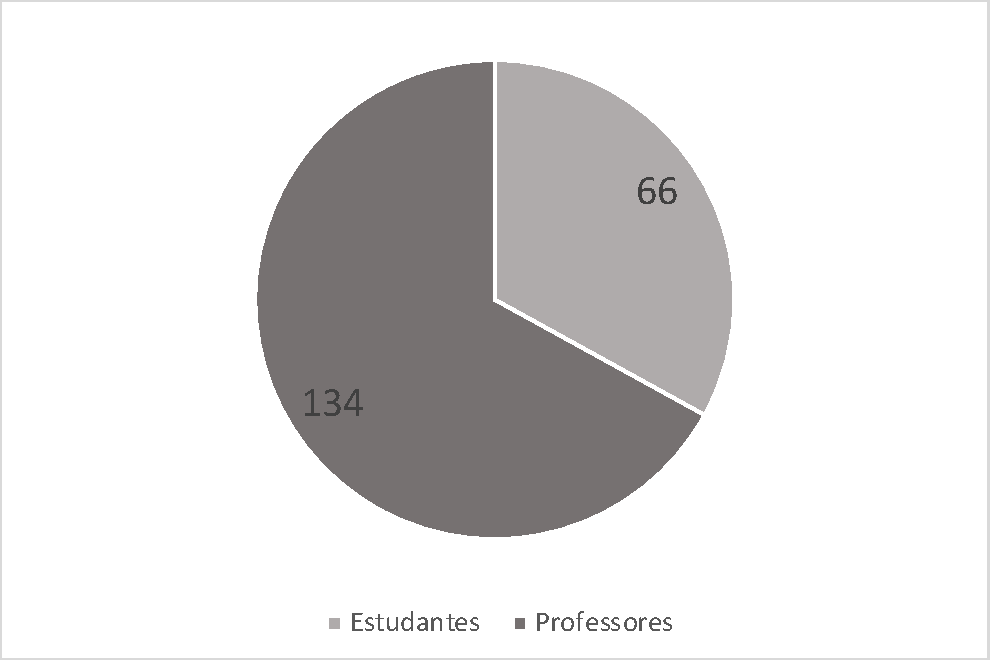
\includegraphics[width=0.85\textwidth]{Figura1.pdf}
 \caption{Perfis 2018.}
 \label{Fig1}
 \source{Dados dos autores.}
\end{figure}

\begin{figure}[htbp]
 \centering
 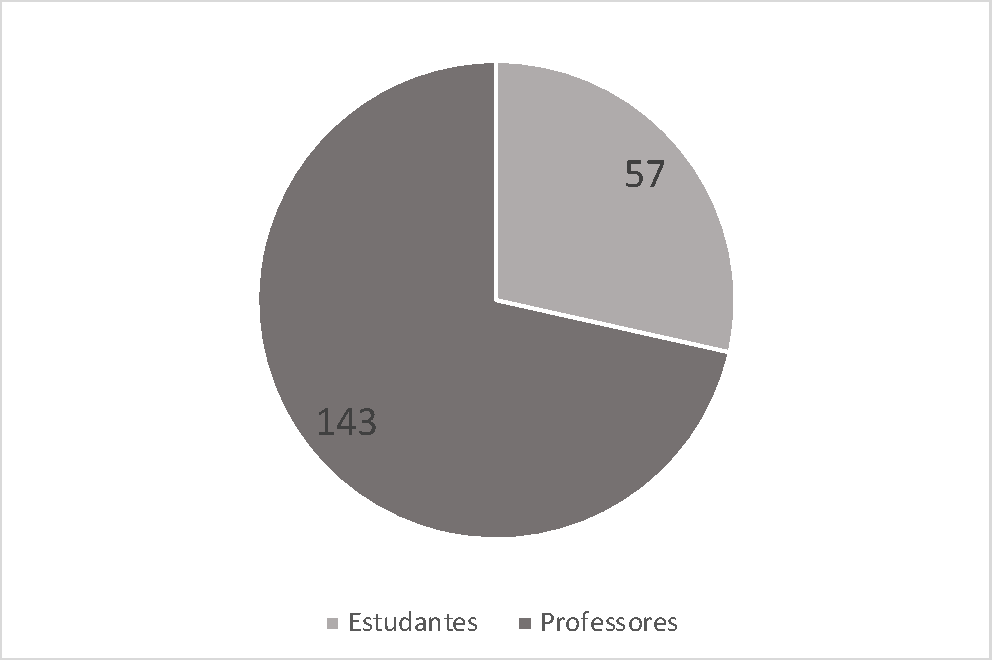
\includegraphics[width=0.85\textwidth]{Figura2.pdf}
 \caption{Perfis 2019.}
 \label{Fig2}
 \source{Dados dos autores.}
\end{figure}

\begin{figure}[htbp]
 \centering
 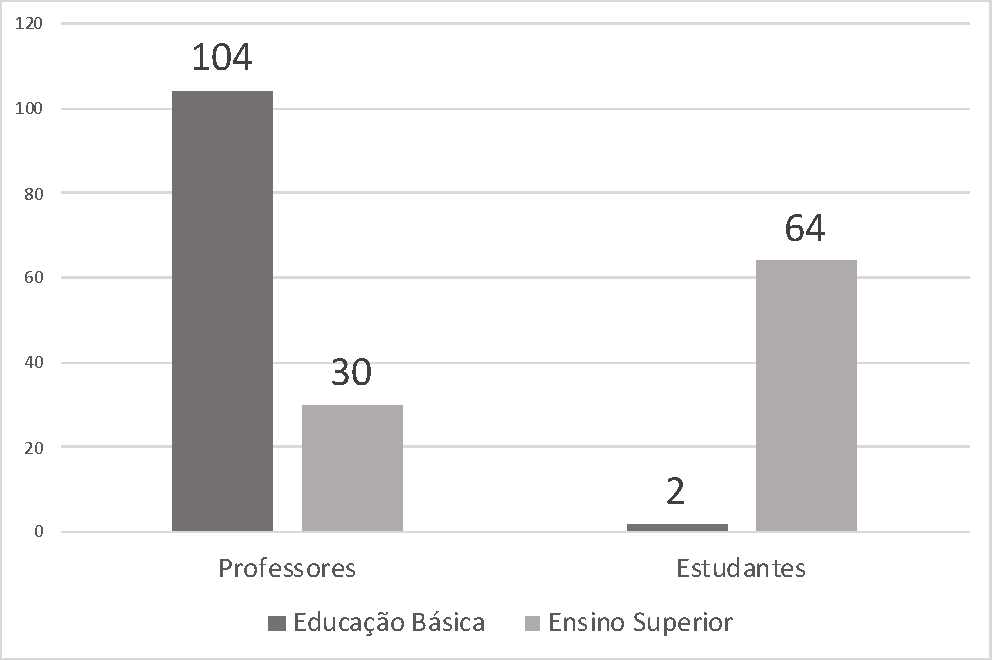
\includegraphics[width=0.85\textwidth]{Figura3.pdf}
 \caption{Contextos escolares 2018.}
 \label{Fig3}
 \source{Dados dos autores.}
\end{figure}

\begin{figure}[htbp]
 \centering
 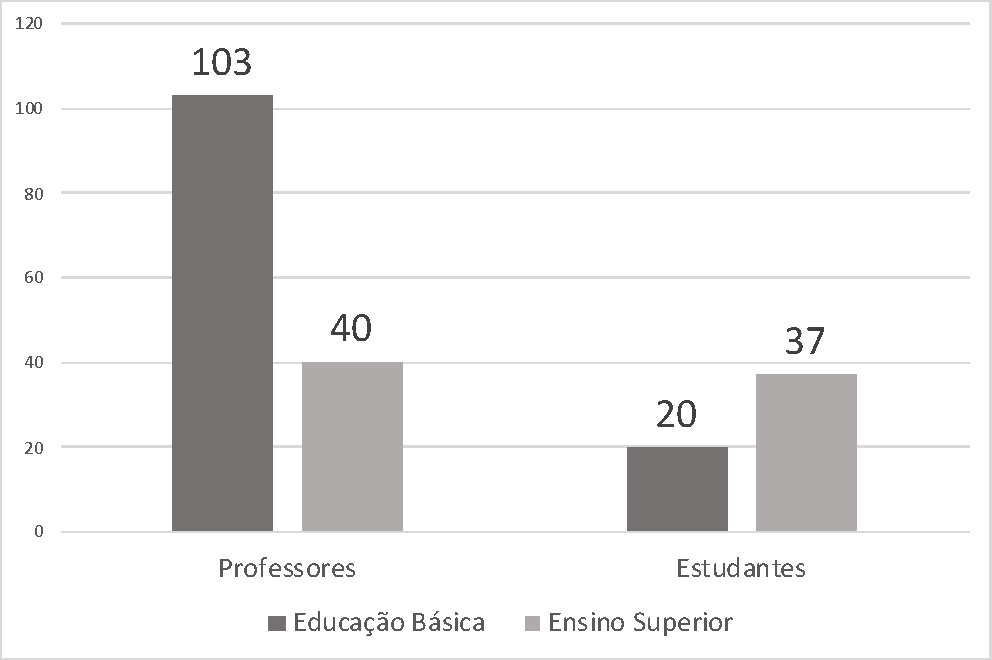
\includegraphics[width=0.85\textwidth]{Figura4.pdf}
 \caption{Contextos escolares 2019.}
 \label{Fig4}
 \source{Dados dos autores.}
\end{figure}

\begin{figure}[htbp]
 \centering
 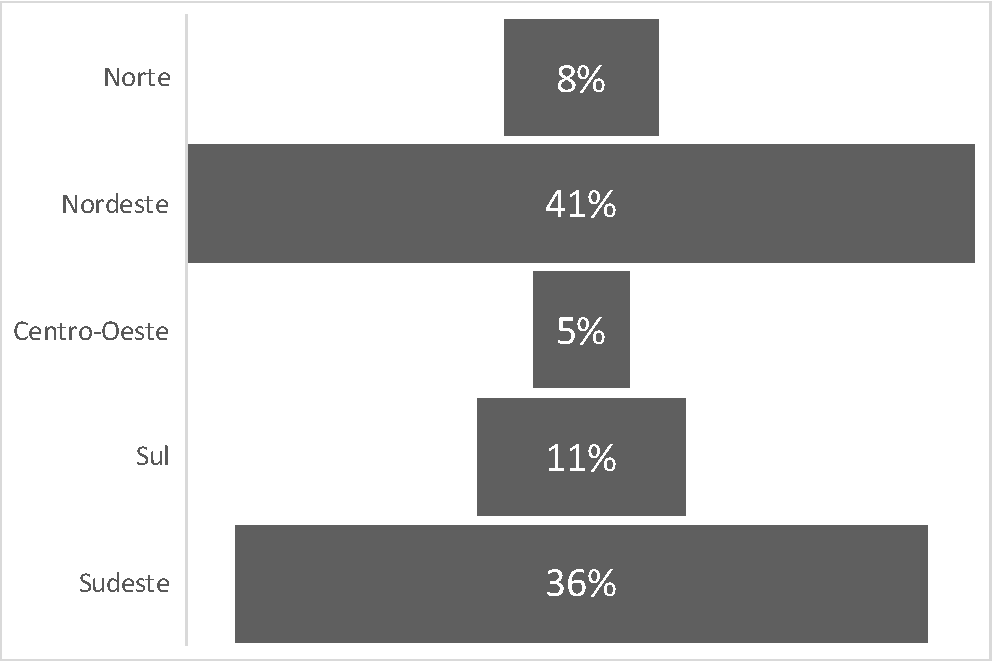
\includegraphics[width=0.85\textwidth]{Figura5.pdf}
 \caption{Regiões 2018.}
 \label{Fig5}
 \source{Dados dos autores.}
\end{figure}

\begin{figure}[htbp]
 \centering
 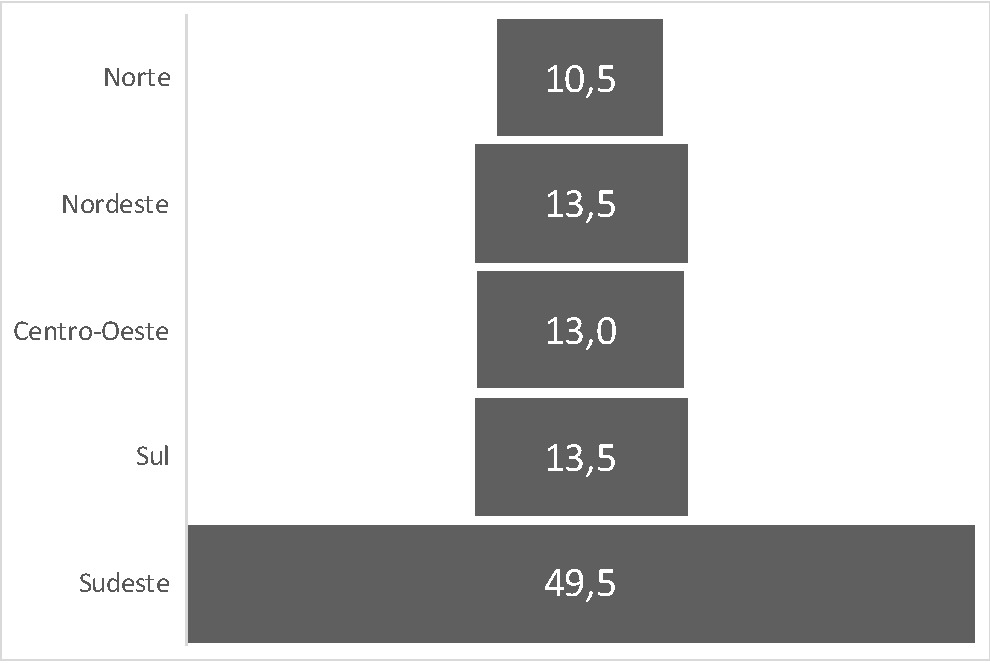
\includegraphics[width=0.85\textwidth]{Figura6.pdf}
 \caption{Regiões 2019.}
 \label{Fig6}
 \source{Dados dos autores.}
\end{figure}

Como ilustram esses gráficos, a grande maioria dos participantes do estudo é formada por professores de inglês da educação básica. Em relação ao contexto de atuação, o questionário apresentava três opções: Ensino Fundamental, Ensino Médio e Ensino Superior, sem fazer distinção entre os setores público e privado. Uma falha no questionário foi não ter incluído escolas de idiomas.

Acreditamos que esta pesquisa pode apresentar um possível panorama do perfil dos estudantes e dos profissionais que ensinam a língua inglesa nas salas de aula do Brasil, bem como suas preferências no que diz respeito aos recursos tecnológicos que usam em suas práticas educacionais, seja dentro ou fora da sala de aula. Isso pode sinalizar, sem generalizações, pontos para discussão e reflexão sobre o uso educacional das tecnologias digitais.

Segundo \textcite{asik_ict_2020}, professores são vistos como pivôs no uso da tecnologia em função das necessidades de seus estudantes e da demanda por engajamento. Isso dialoga com os dados do relatório de Ensino de Inglês na Educação Pública Brasileira \cite{british_council_o_2015}, que revela que os professores percebem os recursos didáticos tecnológicos como altamente relevantes no ensino da língua, muito mais até do que em outras áreas do conhecimento. Isso se dá pelo entendimento de que há uma grande demanda por mais ludicidade e interatividade nas aulas, de modo a motivar e proporcionar mais prática com a língua estudada.

Por outro lado, entendemos que estudantes também contribuem para que professores conheçam novas ferramentas e passem a incorporá-las. Assim, esperamos que os dados aqui analisados contribuam para que novas ideias possam ser incorporadas nas propostas pedagógicas vigentes.


\section{Os recursos digitais utilizados pelos participantes}\label{sec-fmt-manuscrito}
Na parte inicial do questionário, apresentamos alguns recursos comumente utilizados por estudantes e professores em suas práticas docentes e pedimos que os participantes nos informassem se faziam uso deles e em que tipo de dispositivo costumavam acessá-los. Nos dois \textit{surveys}, o uso de dicionários, vídeos e tradutores foram os mais mencionados pelos participantes, sinalizando a presença marcante desses recursos na cultura de ensinar e aprender línguas no Brasil, como ilustram as \Cref{Fig7} e \Cref{Fig8}.

\begin{figure}[htbp]
 \centering
 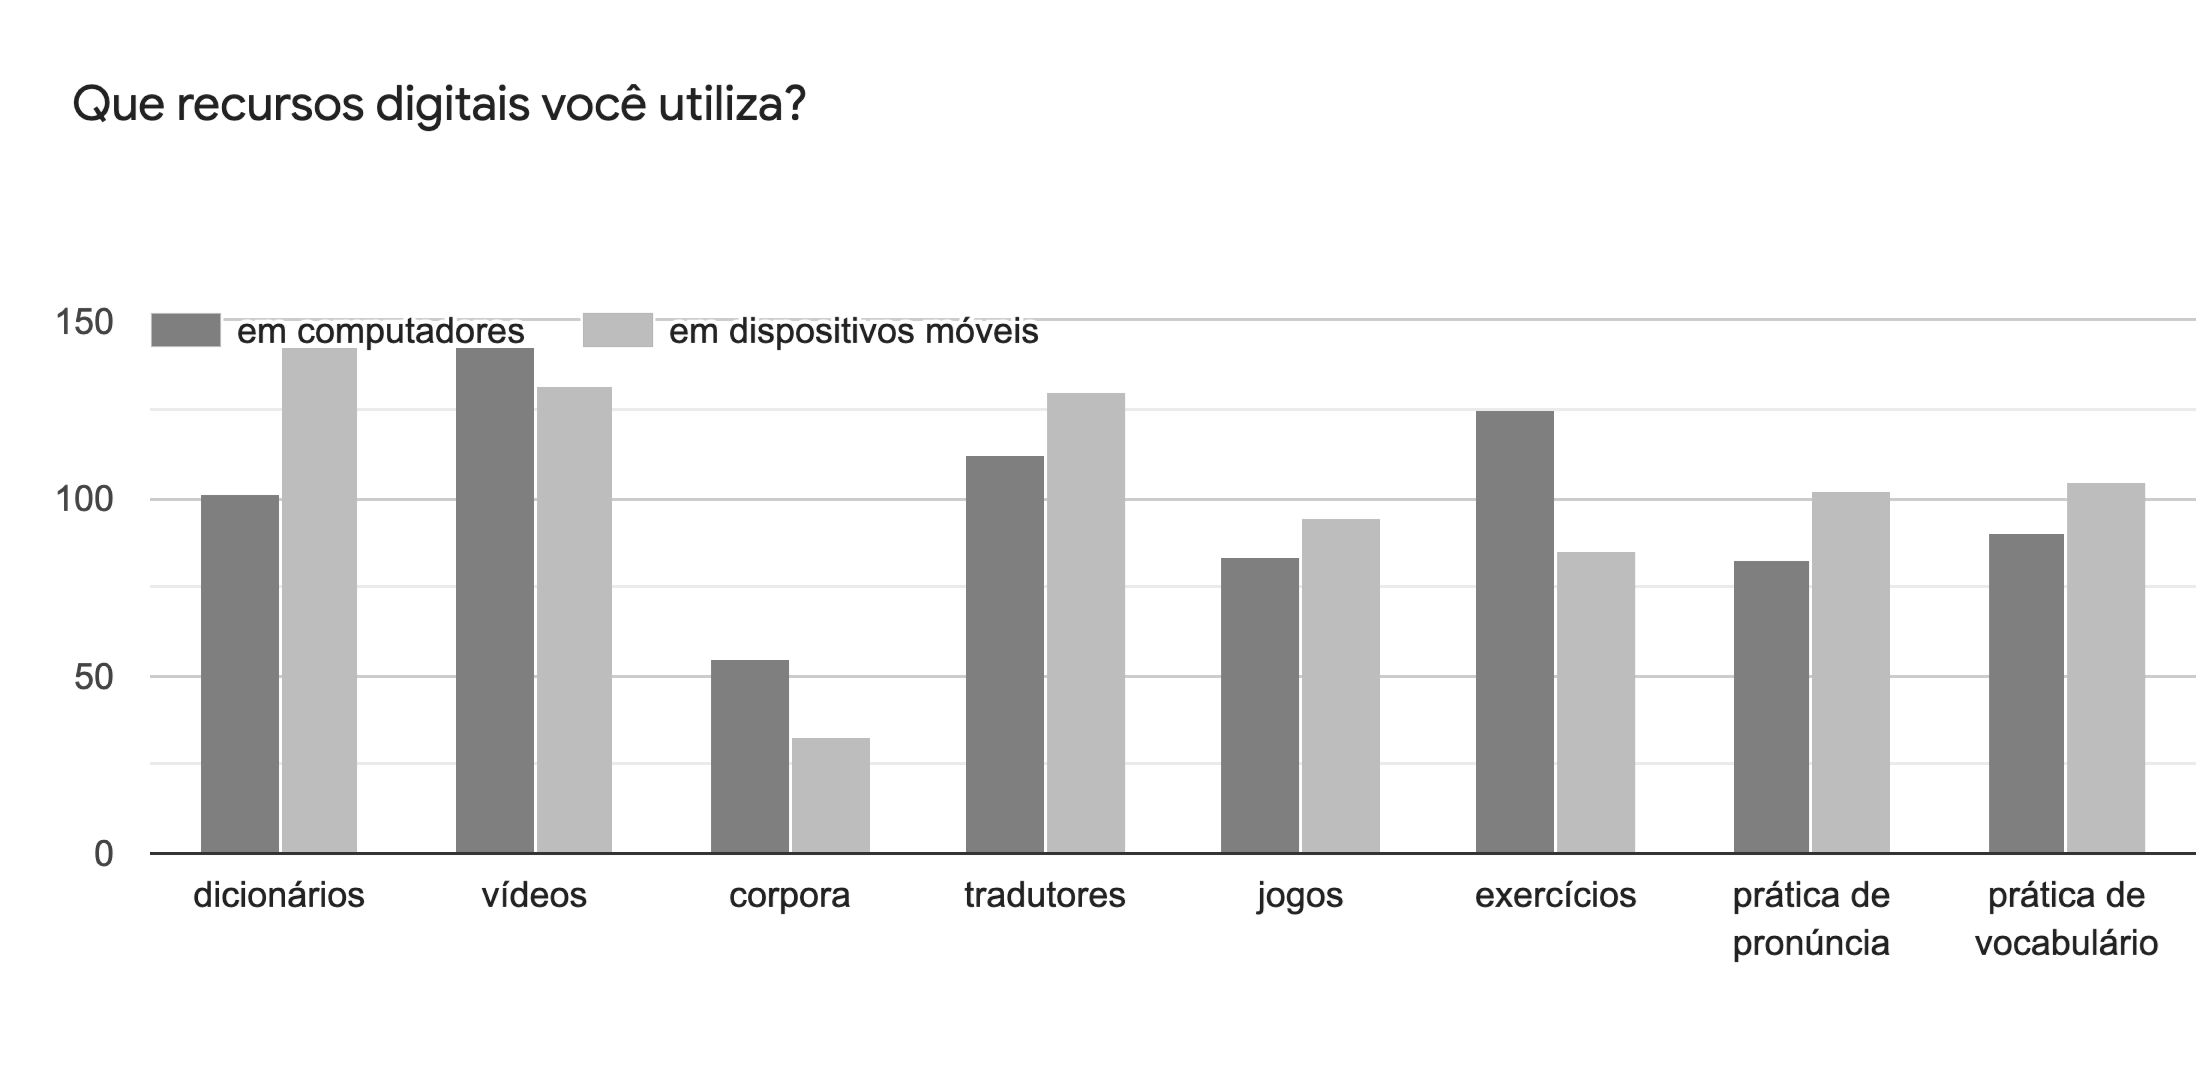
\includegraphics[width=0.85\textwidth]{Figura7.png}
 \caption{Proporção de recursos digitais utilizados pelos participantes em computadores e em dispositivos móveis, em 2018.}
 \label{Fig7}
 \source{Dados dos autores.}
\end{figure}

\begin{figure}[htbp]
 \centering
 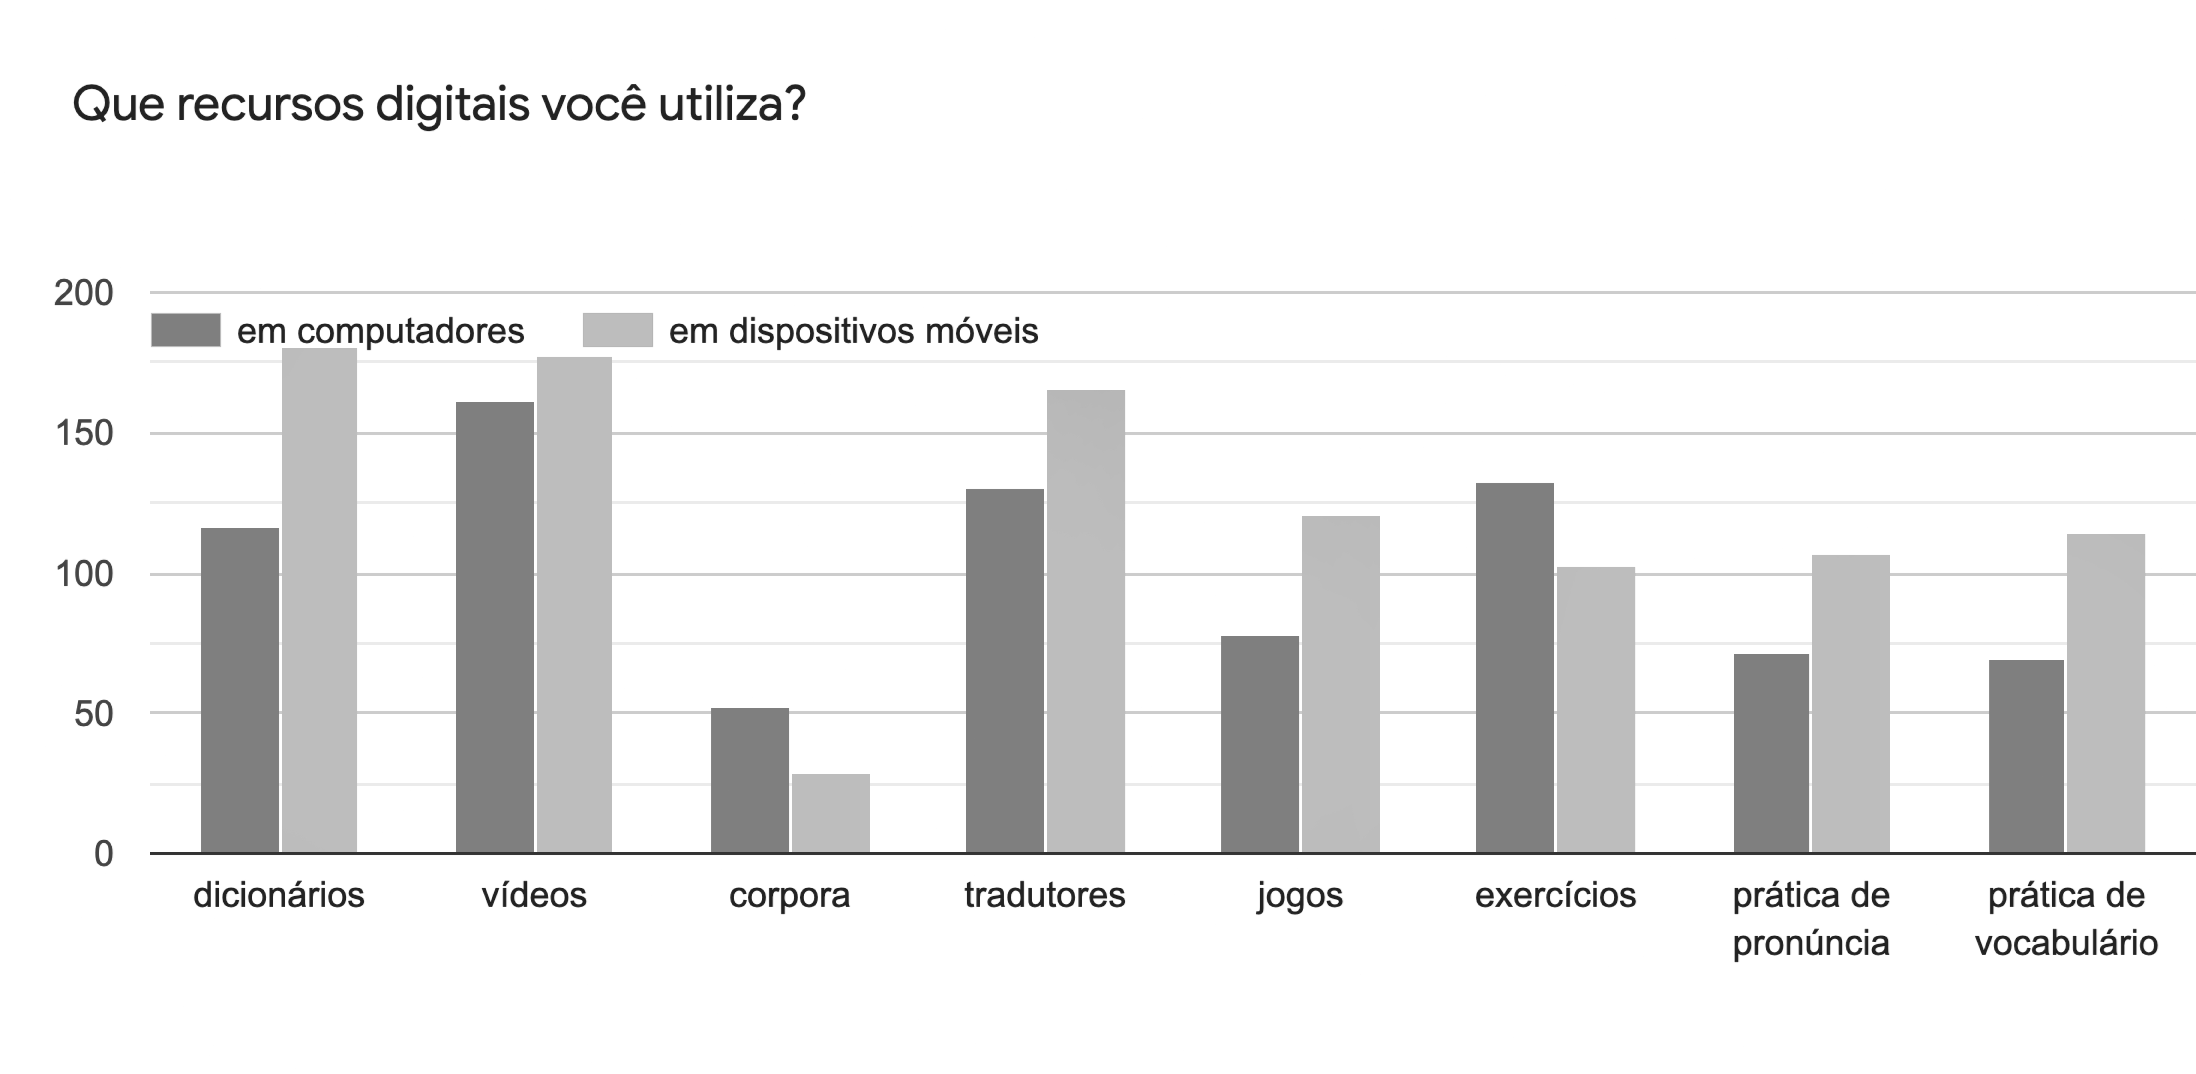
\includegraphics[width=0.85\textwidth]{Figura8.png}
 \caption{Proporção de recursos digitais utilizados pelos participantes em computadores e em dispositivos móveis, em 2019.}
 \label{Fig8}
 \source{Dados dos autores.}
\end{figure}

Como podemos perceber, os participantes parecem reconhecer a oportunidade de acesso ao conhecimento que os recursos digitais oferecem, haja vista a menção significativa do uso de dicionários, tradutores e conteúdos em vídeo. Poderíamos especular que o uso desses recursos é alto por propiciar ações já consolidadas na prática docente que outrora eram mediadas por outras tecnologias, como dicionários (bilíngues e de sinônimos) e livros impressos. No entanto, precisaríamos de mais dados para aprofundamento dessa questão da mediação de recursos digitais nas práticas escolares.

Em relação aos dispositivos utilizados, parece-nos não haver diferença significativa que sinalize preferência por um determinado equipamento. Todavia, percebemos que há certos recursos que são mais acessados em um tipo de dispositivo, como, por exemplo, os jogos nos dispositivos móveis e os exercícios em computadores (sejam eles de mesa ou portáteis). Isso pode estar relacionado à questões de ergonomia e usabilidade, haja vista que o tamanho da tela e das teclas, bem como os demais instrumentos de ação (como o teclado e o mouse), interferem significativamente em nossa interação com as máquinas.

\subsection{A voz dos participantes}\label{sec-formato}
Após esse mapeamento inicial, optamos por deixar um espaço para ouvir os participantes na tentativa de inventariar, de maneira mais específica, as tecnologias digitais utilizadas por eles.

Em 2018, obtivemos 75 respostas (23 estudantes e 52 professores) para a pergunta aberta “Há outros recursos digitais que você utiliza? Se sim, quais?”.

As respostas apontaram para o uso de dicionários específicos; jornais; revistas; determinados sites com atividades para o ensino de inglês; jogos e videogames; \textit{podcasts}; séries e filmes em \textit{streaming}; \textit{e-books}; música, dispositivos digitais, como \textit{tablet} e projetor; WhatsApp; Instagram; Skype; produtos Google; aplicativos móveis; recursos para criação de material didático; ambientes virtuais diversos e algumas mídias, como rádio \textit{on-line}, vídeos no YouTube, e arquivos em formato MP4. Alguns repetiram recursos incluídos na pergunta fechada.  

Em 2019, obtivemos a resposta de 72 participantes para a referida pergunta (15 estudantes e 57 professores). As respostas também mencionaram os recursos digitais indicados no ano anterior, com exceção de projetores, rádio \textit{on-line}, videogame e arquivos em formato MP4. No entanto, outros recursos foram elencados, como o serviço de música em \textit{streaming} Spotify (talvez uma alternativa ao formato MP4), corretores dos pacotes Office ou corretores \textit{on-line} como o Grammarly, ferramentas de busca, editores de texto e redes sociais. Serviços de armazenamento de arquivos nas nuvens foram também citados, bem como programas do pacote Office e ferramentas usadas para criar infográficos e \textit{blogs}. Os respondentes ainda nomearam ferramentas para o acesso a chats, jogos, \textit{blogs}, telecolaboração e ferramentas que são frequentemente usadas em sala de aula, como Edmodo e Kahoot. No questionário do ano de 2019, também houve uma menção ao uso de óculos de realidade virtual por uma professora.
	
Em se tratando do conjunto total de dados, ambos os grupos de participantes mencionaram \textit{podcasts} e filmes. No grupo dos professores houve muitas menções a ferramentas para aulas e para produção de materiais, tais como Canva, Prezi, Slideshow, Google Classroom.  Um dos estudantes disse “acompanhar influenciadores digitais no Instagram para aprender mais”. Skype (“para praticar com pessoas de outro país”) foi mencionado por um aluno e nenhuma menção foi feita no grupo dos professores. Comparando estudantes e professores, verificamos que os dois grupos mencionam aplicativos, músicas, \textit{podcasts}, WhatsApp e vídeos do YouTube. Chamaram nossa atenção as falas de dois/duas professores(as) que alegaram não usar nenhum recurso porque o uso de tecnologia é proibido em suas escolas. Um/a participante em 2019 mencionou o seguinte:

\begin{quote}
    Utilizo o projetor e meus slides. Infelizmente meu contexto não permite o uso de outras tecnologias. Não temos computadores e nem internet. Quando sugiro o uso do celular em aula a coordenação e outros colegas repudiam, pois não acreditam que posso dar aulas utilizando os celulares dos meus alunos. (2019)
\end{quote}

Esta fala condiz com um levantamento do \textcite{british_council_o_2015}, que aponta o projetor de slides como o segundo recurso disponível em sala mais usado (42\%), perdendo apenas para o livro didático. Nesse mesmo levantamento, é possível entender que apenas 24\% dos professores da rede pública tinham acesso à internet nesta época.

Em relação à pergunta seguinte, que solicitava aos informantes que listassem os aplicativos de celular mais usados para aprender ou ensinar inglês, houve uma clara preferência pelo Duolingo (52 pessoas). Esse e os outros recursos mais citados estão listados na \Cref{tbl01}.

\begin{table}[htpb]
\caption{Recursos mais citados em 2018.}
\label{tbl01}
\begin{tabularx}{\linewidth}{XXXX}
\toprule 
\textbf{Recursos}  & \textbf{Estudantes} & \textbf{Professores} & \textbf{Total} \\ 
\midrule
Duolingo & 23 & 29 & 52 \\
Dicionários \textit{on-line} & 11 & 17 & 28 \\
Produtos Google & 6 & 16 & 22 \\
YouTube & 4 & 12 & 16 \\
Kahoot & 3 & 10 & 13 \\
WhatsApp & 3 & 9 & 12 \\
Materiais da BBC & 1 & 6 & 7 \\
Lyrics Training & 1 & 6 & 7 \\
ABA & 2 & 4 & 6 \\
TED & 0 & 5 & 5 \\
Quizlet & 0 & 4 & 4 \\
Babbel & 0 & 3 & 3 \\
Busuu & 0 & 3 & 3 \\
HelloTalk & 2 & 2 & 4 \\
Podcasts & 0 & 4 & 4 \\
\bottomrule
\end{tabularx}
\source{Elaboração dos autores.}
\end{table}

Alguns recursos foram mencionados duas vezes: (Facebook, Hello English, Instagram, Memrise, MosaLinguaEnglish, My English online, Netflix e Tools for Teacher). Outros, incluindo portais, foram citados apenas uma vez. São eles: Alphabear: Words Across Time, Anki, Askjackie, Ask Teacher Lucinia, Audiobooks, Backpacker, British Council, Cambly, Cambridge games, Cambridge readers, Charades, Classdojo, Close Maker, Cloudy, Coursera, Curiosity, Drops, Elsa, English Bites, English Central, English Listening, English Live, EnglishMeo, English Speaking Practice, EngVid, Edx, Edpuzzle, English Town, Grammar Girl, Grammar Safari, ISF (Idiomas sem fronteiras), Italki, Lingdeer, Lessons in life quotes, Lingualeo, OCG to IELTS, Padlet, Phrasal verbs machines, Plickers, Pownton, ToPhonetics, Rosetta Stone, Sentence Master, Skype, Socrative, Spotify, Starfall, Tandem, Trello, Uol, VCE English,Voki, e Wordfun.

Em 2019, 173 participantes responderam a essa pergunta. Novamente, a maioria mencionou o Duolingo (63 pessoas). Veja, na \Cref{tbl02}, os recursos mais citados.

\begin{table}[htpb]
\caption{Recursos mais citados em 2019.}
\label{tbl02}
\begin{tabularx}{\linewidth}{XXXX}
\toprule 
\textbf{Recursos}  & \textbf{Estudantes} & \textbf{Professores} & \textbf{Total} \\ 
\midrule
Duolingo & 20 & 43 & 63 \\
Dicionários & 9 & 32 & 41 \\
Produtos Google & 8 & 27 & 35 \\
Kahoot & 8 & 21 & 23 \\
Recursos da BBC & 3 & 11 & 14 \\
YouTube & 4 & 9 & 13 \\
WhatsApp & 0 & 11 & 11 \\
Lyrics Training & 1 & 6 & 7 \\
Instagram & 1 & 4 & 5 \\
Ted Talks & 1 & 4 & 5 \\
Babbel & 4 & 0 & 4 \\
Cambly & 0 & 4 & 4 \\
Elsa & 0 & 3 & 3 \\
Grammarly & 0 & 3 & 3 \\
Memrise & 0 & 3 & 3 \\
Podcast & 0 & 3 & 3 \\
Tandem & 1 & 2 & 3 \\
\bottomrule
\end{tabularx}
\source{Elaboração dos autores.}
\end{table}

Alguns \textit{apps} foram mencionados duas vezes (Materiais do British Council, Busuu, Canva, English Live, Facebook, IELTS, Netflix, Quizlet, Quiz Your English, Rivet English, Pronunciation Apps, Skype, Spotify,  VOA, Voki, Wordreference), ou apenas uma vez (Aba English, Agendaweb, American English Pronunciation, Anki, Ankidroid,Beelingvo, Castbox, Charades App, CreateWebquest, English Town, Ecaths, ELLO, English Conversation, English Grammar, English Stories, ESL games, Falou, Find words, Forvo, Hello Talk, Idioma sem Fronteiras, Khan academy, LanguageGuide.org, LearnEnglishGrammar, LearnEnglish Sounds Right, Lingualeo. Madlipz, Mendimeter, Moodle, MosaLinguaEnglish, Padlet, Phonetics App, Plickers, Prezi, Reverso Context, Simpler English, Socrative, Readworks, Reddit, Rosetta Stone, Twitter, TOEIC Apps,Tradukka, Voice Spice, Voxy, Web línguas, Weebly, Write \& Improve, Zoom meeting.

Comparamos nossos \textit{surveys} sobre o uso de ferramentas no ensino e aprendizagem de inglês ao estudo conduzido por \textcite{hart_edu100:_nodate}, do \textit{Centre for Learning \& Performance Technologies}, sobre as 100 ferramentas mais usadas na educação superior em 2019. Verificamos que no \textit{survey} de \textcite{hart_edu100:_nodate}, que contou com participantes de 46 países, figuram algumas das ferramentas que se destacam em nossos estudos. Os produtos Google (Google Search; Google Docs; Google Forms) ficaram dentre as dez ferramentas mais citadas; YouTube ocupou o primeiro lugar, e Kahoot o sétimo.

A seguir, apresentamos breves considerações sobre as ferramentas mais citadas, que já foram objeto de investigação por pesquisadores no Brasil e em outros países. Reconhecemos a importância de mostrar como essas ferramentas são empregadas em variados contextos, e como pesquisadores diversos têm observado seus usos e os resultados que elas podem favorecer. No entanto, por questões de espaço, trazemos apenas alguns exemplos mais voltados para o ensino e aprendizagem de inglês, foco deste trabalho, em especial trabalhos realizados no Brasil.

\subsection{Os seis recursos mais mencionados pelos participantes}\label{sec-modelo}
Os recursos mais citados pelos participantes são, também, os que já foram alvo de outras pesquisas em contextos educacionais. Essas pesquisas foram feitas em contexto de aprendizagem de línguas, mas é possível, também, encontrar pesquisas em outras áreas de conhecimento, diferentes da Linguística Aplicada, como na Matemática \cite{romio_kahoot_2017}, na Comunicação Social \cite{anita_baptista_circulacao_2019} e no ensino de Enfermagem \cite{pereira_critical_2016}. Nesta seção, apresentamos os recursos que mais se destacaram dentre os aprendizes e professores neste \textit{survey}, que são: Duolingo, Dicionários on-line, Ferramentas Google, YouTube, WhatsApp e Kahoot.  Ao fazermos isso, citamos pesquisadores que se dedicaram à análise desses recursos e trazemos suas principais considerações.

\subsubsection{Duolingo}\label{sec-organizacao}
O Duolingo mostra-se consideravelmente saliente nas respostas dos participantes e isso coincide com dados de um estudo de \textcite{paiva_aplicativos_2017}, que avaliou quatro aplicativos móveis para aprendizagem de idiomas. O Duolingo é um aplicativo de aprendizagem de idiomas que incorpora recursos e estratégias de gamificação, prometendo, de acordo com seu site oficial, uma aprendizagem “divertida e viciante”. A proposta é avançar por meio da aprendizagem de palavras, frases e estruturas gramaticais, oferecendo recompensas em forma de moedas e desbloqueio de novos níveis. Outras características mencionadas por \textcite{paiva_aplicativos_2017} são: uso do método de gramática-tradução, a presença de ilustrações como apoio para a aprendizagem de vocabulário, arquivos em áudio para auxiliar na pronúncia, e \textit{feedback} multimodal - por exemplo, o uso da palavra “Correto!” acompanhada de um som com efeito alegre.  

Frequentemente, o \textit{app} aparece entre os melhores para se aprender uma língua estrangeira (LE) e seu uso tem se popularizado cada vez mais, como se percebe nos dados gerados nesta pesquisa. Segundo o site oficial, “um estudo demonstrou que 34 horas de Duolingo são equivalentes a um semestre universitário de curso de idioma”. No entanto, em conversas informais e em comentários no fórum da própria ferramenta, é possível perceber que alguns usuários têm consciência de que apenas o Duolingo não é o suficiente para se aprender uma LE. \textcite{paiva_aplicativos_2017} também destaca que a proposta de ensino de vocabulário e de gramática não é contextualizada e tem um caráter mais estrutural, com foco na pronúncia e na tradução.

Estudos têm sido realizados para investigar a eficácia do aplicativo para a aprendizagem de LE. O já citado estudo de \textcite[p. 19]{paiva_aplicativos_2017} ressalta o aspecto gamificado do aplicativo como algo que chama a atenção dos usuários de forma positiva, mas também aponta “a presença de frases e sintagmas nominais improváveis de serem encontrados na linguagem cotidiana”. Dois dos vários exemplos citados pela autora são “I am a turtle” e “Goodbye, elephant”.

O caráter estrutural do aplicativo também foi levantado por \textcite{marques-schafer_concepcoes_2018}. Elas investigam, em um trabalho de base qualitativa-interpretativista, a concepção de aprendizagem de usuários do Duolingo para saber como aprendizes que usam ou já usaram o aplicativo definem suas experiências de aprendizagem de línguas. Partindo de um \textit{corpus} composto por dados coletados por meio de um questionário respondido por aprendizes de línguas estrangeiras, as autoras verificaram que há um desencontro entre o discurso do aplicativo e a prática, bem como uma contradição entre o conceito de aprendizagem dos usuários e seus hábitos. Apesar de citarem, por exemplo, a importância da realização de atividades sócio-interacionais e interculturais para se aprender uma língua, os respondentes destacaram como positivas as tarefas do \textit{app} que não apresentam nenhuma interação (preenchimento de lacunas, tradução de vocabulário, transcrição de palavras e frases, dentre outras).

A pesquisa de mestrado de \textcite{honorato_duolingo_2018} teve como objetivo identificar potencialidades e limitações do aplicativo para o desenvolvimento da competência lexical de aprendizes, inseridos ou não em contexto formal de ensino. A autora se apoiou no campo da Lexicologia Aplicada ao Ensino e da pedagogia crítica centrada no papel do professor como teorizador da própria práxis e realizou uma pesquisa documental em documentos oficiais como os Parâmetros Curriculares Nacionais \cite{brasil_parametros_2000}\footnote{Como a pesquisa foi publicada em 2018, é compreensível que a autora não faça referência à Base Nacional Comum Curricular (BNCC). Esse documento só foi homologado em 2018.} e o Quadro Comum Europeu de Referência para o Ensino de Línguas \cite{conselho_da_europa_quadro_2001}, e uma análise do aplicativo Duolingo. Resultados apontam como pontos positivos a organização das atividades por campos semânticos, a ludicidade e a repetição de exercícios para fixação dos conteúdos. A interface infantilizada, o repertório limitado de vocabulário e a predominância do método gramática-tradução foram destacados como limitações do \textit{app}.

\subsubsection{Dicionários \textit{on-line}}\label{sec-organizacao-latex}
Dicionários \textit{on-line} foram muito citados na coleta feita em 2019, com maior ocorrência do que o Kahoot e o Youtube, inclusive. Eles são recursos potenciais para qualquer aprendiz de idiomas, seja em contexto formal ou informal. Hoje, é possível acessar diferentes dicionários \textit{on-line} por meio de aplicativos para diferentes sistemas operacionais.

\textcite{pereira_o_2017} fez uma revisão bibliográfica com o objetivo de refletir sobre o uso de dicionários impressos e eletrônicos na sala de aula. O trabalho destacou a relevância dos dicionários em formato eletrônico no processo de ensino e aprendizagem da língua inglesa. Essas ferramentas apresentam uma estrutura dinâmica e interativa, que torna mais fácil o acesso e a busca da informação mais imediata. A autora pondera que o dicionário eletrônico surge como uma importante ferramenta pedagógica no sentido de conectar o ensino de Língua Inglesa à cultura digital.

A ferramenta Linguee, também muito citada na coleta feita em 2019, faz parte do grupo de dicionários \textit{on-line}, mas com uma característica particular: ela também é um \textit{corpus} paralelo, ou seja, ela busca exemplos variados de frases em bancos de dados \textit{on-line} para que o usuário tenha acesso a exemplos reais com suas respectivas traduções. \textcite{aguiar_desafios_2018} observou que, quando o termo é encontrado, “aproximadamente 60\% dos links são de sites acessíveis”, o que possibilita verificar a confiabilidade das fontes. Em outra pesquisa, o Linguee foi utilizado por \textcite{grespan_escrita_2017} para verificar inadequações vocabulares em textos acadêmicos de alunos do 1º ano de um curso de Secretariado Executivo. O dicionário foi utilizado para confirmar se havia mesmo inadequação de uso de vocabulário em alguns trechos das redações por ela corrigidas.

\subsubsection{Ferramentas Google}\label{sec-titulo}
As ferramentas Google possuem diversas funções importantes para o nosso fazer diário e na educação não poderia ser diferente: busca de informações para pesquisas escolares (Google search engine); uso do tradutor em sala de aula ou em outro contexto para acesso à tradução e/ou pronúncia de frases e palavras; busca de imagens para fins de ilustração de algum vocabulário específico; uso do espaço de armazenamento do Google Drive;  uso do Google Docs e Google Forms para criar atividades colaborativas e de pesquisa; e uso do Hangouts para videoconferências em língua estrangeira.

Dentre as ferramentas mencionadas, é possível encontrar maior ocorrência de pesquisas voltadas para o uso do Google Docs no contexto educacional. Dentre os vários trabalhos encontrados, destacamos aqui o trabalho de \textcite{santiago_google_2014}. As autoras investigaram o grau de letramento digital dos discentes e suas interações em uma atividade colaborativa da disciplina de língua inglesa instrumental por meio das ferramentas do Google Drive, com preferência de uso pelo editor, o Google Docs. A pesquisa teve uma abordagem qualitativa e os dados foram coletados ao longo de aulas de língua inglesa. Os resultados obtidos sugerem desenvolvimento de habilidades colaborativas, de letramento digital e de melhoria na produção linguística.

Igualmente importante é o trabalho de \textcite{weissheimer_aplicativos_2017}. As autoras investigaram o impacto da escrita colaborativa mediada pelo Google Docs sobre o desenvolvimento da acurácia gramatical de aprendizes de inglês em uma universidade federal brasileira. Os aprendizes investigados vivenciaram uma experiência híbrida de escrita colaborativa de \textit{flash fiction}\footnote{Histórias muito curtas, também chamadas de nanocontos.} e as impressões dos participantes sobre a experiência foram coletadas por meio de um questionário. Os dados quantitativos, segundo os autores, apontaram para um aumento no nível de acurácia gramatical dos estudantes ao longo do semestre e também mostraram a utilidade da escrita colaborativa mediada pela tecnologia no ensino e aprendizagem de LE.

A pesquisa de \textcite{gartner_por_2016} descreve e interpreta o fenômeno da escrita colaborativa em inglês desenvolvida em ambiente \textit{on-line}, usando a tecnologia do Google Docs por estudantes do 9º ano do Ensino Fundamental. O estudo investigou a realização de duas tarefas de escrita em língua inglesa durante as aulas regulares de inglês, de forma síncrona e assíncrona, presencial e a distância. Os resultados evidenciaram que a escrita colaborativa no meio digital pode contribuir para a concepção e aplicação de projetos colaborativos com foco na escrita em língua estrangeira. Foi possível perceber também, segundo o autor, que podem ser desenvolvidas capacidades de comunicação e cooperação com ajuda da tecnologia, bem como o pensamento crítico com o apoio um ambiente de aprendizagem propício à interação.

\subsubsection{WhatsApp}\label{sec-autores}
O aplicativo WhatsApp tem sido usado por estudantes e professores, tanto para comunicação geral quanto para atividades relacionadas à aprendizagem de línguas. Na Universidade Federal de Minas Gerais (UFMG), o projeto Taba Eletrônica já ofertou cursos de formação continuada totalmente \textit{on-line} para o uso do WhatsApp nas aulas de inglês, propondo tarefas para os participantes se engajarem com a ferramenta em seus usos pedagógicos. Desse projeto, foram publicados artigos com resultados das pesquisas realizadas a partir dessas formações de professores \cite{braga_aprendizagem_2017,braga_reflexoes_2017}.

Pesquisas de mestrado como a de \textcite{boechat_o_2019} trazem resultados do uso do WhatsApp por alunos do ensino fundamental. De maneira geral, o uso do WhatsApp voltado para ensino e aprendizagem de inglês remete à oportunidade de interação entre professores e aprendizes, dentro de um desenho pedagógico apropriado, onde quer que eles estejam. Dentre os resultados destacados na pesquisa, o uso autêntico do idioma, especialmente no uso do recurso de gravação de áudio, é o que mais chama a atenção no uso pedagógico da ferramenta.

\textcite{teixeira_formacao_2018} concluiu que o uso das tecnologias móveis trouxe mais possibilidades para expandir o acesso de docentes às oportunidades de formação continuada. Essa opção configura-se como um ponto de partida para uma aproximação dos professores com o uso de dispositivos e aplicativos móveis no contexto de línguas e para a discussão e reflexão sobre os potenciais e as limitações dessas tecnologias no espaço escolar.

Uma das questões que precisam ser mais debatidas refere-se ao fato de que ao mesmo tempo em que essas tecnologias digitais flexibilizam as noções de tempo e espaço, elas podem contribuir para um rompimento com a distinção entre tempo de trabalho e descanso do professor.

\subsubsection{Kahoot}\label{sec-idioma}
O Kahoot é uma plataforma gratuita que facilita a criação e o compartilhamento de jogos ou trivias, que podem ser usados na escola, no trabalho ou em casa. Seu aspecto gamificado do Kahoot parece gerar envolvimento dos participantes nos jogos, o que faz com que venha ser objeto de pesquisas na área da educação de línguas.

\textcite{bottentuit_junior_o_2017}, em artigo bibliográfico e descritivo, enxerga no aplicativo a possibilidade de estímulo do engajamento dos alunos.  O autor elencou as vantagens da ferramenta na educação, como o aumento da motivação dos alunos; a melhoria do raciocínio e da concentração nas aulas; as possibilidades de inversão de papéis e trabalho colaborativo; e a avaliação da aprendizagem em tempo real. Após um apanhado de vários estudos, ele concluiu que o Kahoot pode se constituir como uma ferramenta educativa e que, por meio dela, é possível incentivar o interesse do aluno para a aprendizagem e melhorar as práticas pedagógicas na sala de aula.

\textcite{weissheimer_aplicativos_2017} realizaram uma pesquisa de natureza mista (qualitativa e quantitativa) com foco na gamificação. Os resultados apontam para o impacto positivo de práticas gamificadas com o Kahoot na aprendizagem de inglês como L2. As pesquisadoras compararam dois grupos, sendo que um deles realizou as atividades no livro didático, de forma não-gamificada. Elas identificaram aumento na motivação e no rendimento acadêmico do grupo que usou o Kahoot ao longo do curso. Além disso, os alunos mencionaram a diversão e a formação de memórias e ainda concluíram que as atividades usando Kahoot se configuram como uma proposta pedagógica engajadora.

\subsubsection{YouTube}\label{sec-resumo}
Outra ferramenta muito citada nesta pesquisa é o YouTube. A plataforma de compartilhamento de vídeos parte do princípio de que “todos têm o direito de expressar opiniões e que o mundo se torna melhor quando ouvimos, compartilhamos e nos unimos por meio das nossas histórias” \cite{youtube_about_nodate}. A infinidade de materiais postados, em diferentes línguas, permite que aprendizes de línguas tenham acesso a insumo da língua alvo (fidedignos ou não) em variadas situações.

De acordo com \textcite{moran_ensino_2013}, conteúdos audiovisuais são formas de comunicação multissensorial, com mensagens que facilitam a interação com o público. A linguagem audiovisual, segundo esse autor, desenvolve diferentes atos de percepção e seu uso permite que um “expectador” utilize mais de um sentido no processo do assistir e aprender, envolvendo-se mais com o objeto de estudo. O uso de recursos audiovisuais também está associado à vivência de uma experiência significativa e ao uso de material autêntico \cite{geddes_video_1982,mcgill_ten_2010}, que podem atrair o aprendiz e promover resultados de aprendizagem mais favoráveis. Por essas razões, o YouTube pode ter sido tão citado como ferramenta de uso pelos participantes de nossa pesquisa.

\textcite{caetano_you_2007} analisaram a plataforma como uma opção para repositório de material para a educação a distância. Eles apontaram que as possibilidades de utilização são várias, como por exemplo: em \textit{coursewares}\footnote{Materiais digitais desenvolvidos exclusivamente para contextos educacionais.}, em tutoriais, como material de apoio, como portfólio do aluno ou até mesmo como uma TV educacional.

A pesquisa de cunho qualitativo de \textcite{silva_contribuicoes_2018} explorou as contribuições pedagógicas do YouTube para o ensino e aprendizagem de língua estrangeira. Por meio de um \textit{survey} e uma pesquisa documental de base netnográfica do canal do YouTube English in Brasil, o trabalho teve como objetivos (a) compreender e problematizar as possibilidades e desafios que o uso da rede social YouTube trazem ao ensino e aprendizagem de língua estrangeira na educação básica; (b) explorar as habilidades necessárias a professores e alunos para utilizar as redes sociais no ensino e aprendizagem de língua estrangeira; (c) investigar como a formação de professores pode se beneficiar desse tipo de ferramenta; e (d) entender como se dá a participação da audiência de um canal do YouTube voltado para o ensino de língua estrangeira. Segundo a autora, os resultados “mostraram que o YouTube abre um espaço comum para participação ampla e construção colaborativa de conhecimento, já que esse espaço é propício para a interação, comunicação e colaboração” \cite[p. 146]{silva_contribuicoes_2018}. 

\section{Considerações finais}\label{sec-secoes}
A análise dos dados nos mostrou que, já em um momento pré-pandêmico, os participantes demonstravam reconhecer as oportunidades e potencialidades de recursos tecnológicos para aprender e ensinar línguas, o que evidencia que o uso da tecnologia digital já era uma prática consolidada em suas experiências de alguma forma. Sobre o modo como esse uso acontecia, percebemos que certas ferramentas estavam mais associadas a computadores e outras a dispositivos móveis; e isso nos pareceu estar relacionado à questões de ergonomia e usabilidade. Em outras palavras, não basta pensar nas funções das tecnologias; é preciso pensar na experiência do usuário. Essa é uma questão importante a ser considerada em nossas propostas educacionais, haja vista que a sensação de conforto na interação com o dispositivo pode impactar positiva ou negativamente na ação de aprendizagem.

Ao analisarmos as práticas dos participantes, observamos uma desmaterialização da tecnologia propiciada pelo crescimento da computação em nuvem. Nossos resultados revelam, por exemplo, que os videogames e arquivos em formato MP4 vinham sendo menos utilizados pelos participantes da pesquisa. Provavelmente, os videogames estão sendo substituídos pelos jogos \textit{on-line} e os arquivos MP4 pelas plataformas de \textit{streaming}. Acreditamos que essa é uma questão a ser mais explorada em pesquisas na área, haja vista que nossas práticas individuais e sociais estão cada dia mais virtualizadas.

Sobre as ferramentas mais regulares nas respostas dos participantes, percebemos a presença de recursos que foram primariamente desenvolvidas para fins educacionais, como Duolingo, Kahoot e Linguee; e também de tecnologias desenvolvidas para outros fins, mas que também podem ser utilizadas para ensinar e aprender, como as Ferramentas Google, WhatsApp e YouTube. É nosso entendimento que, para promover práticas contemporâneas de ensino e aprendizagem de línguas, é necessário valorizar o \textit{mindset} digital e não apenas investir em ferramentas digitais de última geração.

Como revela este estudo, o ensino e aprendizagem de inglês é uma atividade em que o uso de tecnologias digitais já era, de alguma forma, institucionalizado. No entanto, em um país de proporções continentais como o Brasil, com altos índices de desigualdade social e um evidente abismo digital (potencializado ainda mais pela pandemia), reconhecemos a necessidade de estudos que se proponham a investigar os contextos pandêmicos e pós-pandêmicos (quando possível, evidentemente); para que possamos reconhecer os possíveis outros e novos usos e recursos tecnológicos para ensinar e aprender línguas. Com a presença cada vez mais ubíqua da tecnologia digital, nossa vida se torna cada vez mais fluida, inconstante e não linear. Por isso, acreditamos que devemos estimular a capacidade para observar a tecnologia, extrair o seu valor e aplicá-la em nossos afazeres diários. Não se trata apenas dos usos, mas dos nossos pensamentos e comportamentos, que nos fazem perceber as oportunidades que as tecnologias ao nosso alcance oferecem.


\printbibliography\label{sec-bib}
% if the text is not in Portuguese, it might be necessary to use the code below instead to print the correct ABNT abbreviations [s.n.], [s.l.]
%\begin{portuguese}
%\printbibliography[title={Bibliography}]
%\end{portuguese}


%full list: conceptualization,datacuration,formalanalysis,funding,investigation,methodology,projadm,resources,software,supervision,validation,visualization,writing,review
\begin{contributors}[sec-contributors]
\authorcontribution{Ronaldo Corrêa Gomes Junior}[datacuration,formalanalysis,writing,review]
\authorcontribution{Luciana de Oliveira Silva}[datacuration,formalanalysis,writing,review]
\authorcontribution{Vera Lúcia Menezes de Oliveira e Paiva}[projadm,methodology,supervision,funding,writing,review]
\end{contributors}

\end{document}
